\chapter{Potencial químico e misturas}\label{ch:b2:chemical-potential}

No inverno, um caminhão espalha sal em uma estrada congelada e o gelo
derrete a \qty{-10}{\celsius}; o fluido de arrefecimento de um motor de
carro, água com um terço de etano-1,2-diol, não congela na geada da noite
nem ferve sob um capô quente. Uma substância dissolvida abaixa o ponto de
congelamento de seu solvente e eleva seu ponto de ebulição e, em soluções
diluídas, de um valor que depende do número de partículas dissolvidas e não
de sua natureza. A ferramenta que explica isso é o \omterm{def:b2:chemical-potential:chemical-potential}{potencial químico}, a
derivada parcial da \omterm{def:b2:reaction-free-energy:gibbs-energy}{energia de Gibbs} em relação à quantidade de um
constituinte. Ele diz para onde cada espécie ``quer ir'', entre fases e por
meio de reações, e transforma as atividades que o volume do 1.º ano usava
como receitas em grandezas deduzidas.

\begin{recall}
\Cref{ch:b2:reaction-free-energy}: a \omterm{def:b2:reaction-free-energy:gibbs-energy}{energia de Gibbs} $G = H - TS$, $\dd G =
V\dd p - S\dd T + \Delta_r G\,\dd\xi$, o critério de evolução $\Delta_r G\,
\dd\xi \leq 0$. O volume do 1.º ano escreveu a atividade de um gás como
$p_i/p^\circ$, a de um soluto como $c_i/c^\circ$, e 1 para um sólido puro ou
um solvente, e observou que, em soluções iônicas concentradas, as atividades
se afastam das concentrações, ``uma correção tratada no volume do 2.º ano''.
Da física: a lei dos gases perfeitos e $(\partial G/\partial p)_T = V$ para
uma substância pura.
\end{recall}

\begin{omfigure}

\includegraphics[width=0.58\linewidth]{images/book3/ai/b2-03-salt-spreader.jpg}

{\small Um caminhão espalha sal em uma estrada coberta de neve. O sal se
dissolve na fina película de água sobre o gelo, e a solução congela a uma
temperatura mais baixa que a água pura: o gelo derrete.}
\end{omfigure}

\section{Grandezas parciais molares}

Misture \qty{50}{mL} de água e \qty{50}{mL} de etanol: o volume da mistura
é menor que \qty{100}{mL}. Em uma mistura, uma grandeza extensiva não é a
soma das contribuições das substâncias puras; cada constituinte contribui
de acordo com o que o cerca.

\begin{definition}[Grandeza parcial molar]\label{def:b2:chemical-potential:partial-molar}
Seja $X(T, p, n_1, \dots, n_k)$ uma função de estado extensiva de uma fase
que contém as quantidades $n_1, \dots, n_k$. A \emph{grandeza parcial
molar}\index{grandeza parcial molar} do constituinte $i$ é
\[
  \bar X_i = \left(\frac{\partial X}{\partial n_i}\right)_{T, p, n_{j \ne i}} ,
\]
a variação de $X$ por mol de $i$ adicionado a uma grande quantidade da
mistura, a $T$, $p$ e demais quantidades fixos. Para $X = V$, é o \emph{volume
parcial molar}\index{volume parcial molar} $\bar V_i$.
\end{definition}

\begin{theorem}[Identidade de Euler]\label{thm:b2:chemical-potential:euler}
A $T$ e $p$ fixos, $X = \sum_i n_i\bar X_i$.
\end{theorem}

\begin{proof}
$X$ é extensiva: multiplicar todas as quantidades por $\lambda$ multiplica $X$ por
$\lambda$, isto é, $X(T, p, \lambda n_1, \dots, \lambda n_k) = \lambda X(T, p, n_1,
\dots, n_k)$. Derive em relação a $\lambda$ em $\lambda = 1$, pela
regra da cadeia: $\sum_i n_i\,\partial X/\partial n_i = X$.
\end{proof}

\begin{proposition}[Relação de Gibbs--Duhem]\label{prop:b2:chemical-potential:gibbs-duhem}
A $T$ e $p$ fixos, $\sum_i n_i\,\dd\bar X_i = 0$: em uma mistura binária,
$x_1\dd\bar X_1 + x_2\dd\bar X_2 = 0$. As \omterm{def:b2:chemical-potential:partial-molar}{grandezas parciais molares} dos
constituintes não podem variar independentemente.
\end{proposition}

\begin{proof}
A $T$, $p$ fixos, $\dd X = \sum_i\bar X_i\dd n_i$ por definição; a identidade
de Euler, diferenciada, dá $\dd X = \sum_i\bar X_i\dd n_i + \sum_i
n_i\dd\bar X_i$. Subtraia.
\end{proof}

\begin{omfigure}
\begin{tikzpicture}
\begin{axis}[
  width=0.62\linewidth, height=5.4cm, xmin=0, xmax=1, ymin=8, ymax=62,
  axis x line=bottom, axis y line=left, xlabel={fração molar $x_2$},
  ylabel={volume molar $V_m$ (modelo)}, xtick={0,0.2,0.4,0.6,0.8,1}, ytick=\empty,
  tick label style={font=\small}, label style={font=\small}, ylabel shift=10pt, clip=false]
\addplot[omDef, very thick, domain=0:1, samples=60] {18*(1-x) + 58*x - 25*x*(1-x)};
\addplot[black!40, dashed, domain=0:1] {18*(1-x) + 58*x};
\addplot[omThm, thick, domain=0:1] {14 + 35*x};
\fill[omThm] (axis cs:0.4,28) circle (1.6pt);
\node[omThm, anchor=east, font=\small] at (axis cs:-0.01,14) {$\bar V_1$};
\node[omThm, anchor=west, font=\small] at (axis cs:1,49) {$\bar V_2$};
\node[font=\scriptsize, anchor=south east, black!60] at (axis cs:0.62,44) {soma dos volumes puros};
\node[font=\small, anchor=north west] at (axis cs:0.41,27) {$x_2 = 0.4$};
\end{axis}
\end{tikzpicture}

{\small A construção da tangente. O volume molar de uma mistura binária modelo
(em azul) fica abaixo da reta que une os volumes puros: a mistura se
contrai. A tangente em uma composição corta as duas bordas nos \omterm{def:b2:chemical-potential:partial-molar}{volumes
parciais molares} $\bar V_1$ e $\bar V_2$ dessa composição.}
\end{omfigure}

\begin{method}[Grandezas parciais molares a partir de uma curva]\label{met:b2:chemical-potential:tangent}
Trace a grandeza molar $X_m = X/(n_1 + n_2)$ em função de $x_2$. Na
composição de interesse, trace a tangente: ela corta o eixo $x_2 = 0$ em
$\bar X_1$ e o eixo $x_2 = 1$ em $\bar X_2$. (Demonstração: $X_m = x_1\bar X_1 +
x_2\bar X_2$ e, por Gibbs--Duhem, $\dd X_m/\dd x_2 = \bar X_2 - \bar X_1$.)
\end{method}

\section{O potencial químico}

\begin{definition}[Potencial químico]\label{def:b2:chemical-potential:chemical-potential}
O \emph{potencial químico}\index{potencial quimico@potencial químico} do constituinte $i$ em
uma fase é sua \omterm{def:b2:reaction-free-energy:gibbs-energy}{energia de Gibbs} parcial molar,
\[
  \mu_i = \left(\frac{\partial G}{\partial n_i}\right)_{T, p, n_{j\ne i}} ,
\]
em \unit{J/mol}. Seu valor quando $i$ está em seu estado padrão é seu
\emph{potencial químico padrão}\index{potencial quimico padrao@potencial químico padrão}
$\mu_i^\circ(T)$, igual à \omterm{def:b2:reaction-free-energy:gibbs-energy}{energia de Gibbs} molar padrão de $i$.
\end{definition}

Para uma fase cujas quantidades podem variar (por reação, ou por troca com
outra fase),
\[
  \dd G = V\dd p - S\dd T + \sum_i\mu_i\,\dd n_i ,\qquad G = \sum_i n_i\mu_i ,
\]
a segunda relação pela identidade de Euler. Com uma única reação, $\dd n_i =
\nu_i\dd\xi$ e, comparando com a \cref{prop:b2:reaction-free-energy:dG}:
\[
  \Delta_r G = \sum_i\nu_i\mu_i .
\]
A \omterm{def:b2:reaction-free-energy:reaction-gibbs}{energia de Gibbs de reação} é o balanço dos \omterm{def:b2:chemical-potential:chemical-potential}{potenciais químicos} dos
produtos e dos reagentes.

\begin{theorem}[Equilíbrio entre fases]\label{thm:b2:chemical-potential:phase-equilibrium}
Um constituinte presente em duas fases $\alpha$ e $\beta$ de um sistema fechado a
$T$ e $p$ uniformes está em equilíbrio entre elas se, e somente se,
$\mu_i^\alpha = \mu_i^\beta$. Caso contrário, ele passa espontaneamente da
fase em que seu \omterm{def:b2:chemical-potential:chemical-potential}{potencial químico} é maior para a fase em que ele é menor.
\end{theorem}

\begin{proof}
A transferência $i^\alpha \to i^\beta$ é uma ``reação'' com $\nu^\alpha = -1$,
$\nu^\beta = +1$, logo $\Delta_r G = \mu_i^\beta - \mu_i^\alpha$. Pelo
critério de evolução, ela avança ($\dd\xi > 0$) somente se $\mu_i^\beta <
\mu_i^\alpha$, recua se $\mu_i^\beta > \mu_i^\alpha$, e está em
equilíbrio se forem iguais.
\end{proof}

O \omterm{def:b2:chemical-potential:chemical-potential}{potencial químico} desempenha para a matéria o papel que a temperatura
desempenha para o calor: o calor flui do quente para o frio, uma espécie de
onde seu $\mu$ é alto para onde ele é baixo.

\section{Sistemas ideais e atividades}

\begin{proposition}[Potencial químico de um gás perfeito]\label{prop:b2:chemical-potential:mu-gas}
Em uma mistura de gases perfeitos, um gás de pressão parcial $p_i$ tem
\[
  \mu_i = \mu_i^\circ(T) + RT\ln\frac{p_i}{p^\circ} .
\]
\end{proposition}

\begin{proof}
Para um mol de gás perfeito puro, $(\partial\mu/\partial p)_T = V_m =
RT/p$; integrando de $p^\circ$ a $p$, obtém-se $\mu = \mu^\circ + RT\ln(p/p^\circ)$.
Em uma mistura de gases perfeitos, cada gás se comporta como se estivesse
sozinho no volume, à sua pressão parcial: substitua $p$ por $p_i$.
\end{proof}

\begin{definition}[Mistura ideal, solução diluída ideal]\label{def:b2:chemical-potential:ideal-mixture}
Uma mistura líquida (ou sólida) é uma \emph{mistura ideal}\index{mistura ideal}
se, para todo constituinte e toda composição,
$\mu_i = \mu_i^*(T, p) + RT\ln x_i$, em que $\mu_i^*$ é o \omterm{def:b2:chemical-potential:chemical-potential}{potencial químico}
do líquido puro $i$. Uma solução é uma \emph{solução diluída
ideal}\index{solucao diluida ideal@solução diluída ideal} se o solvente obedece a essa lei e cada
soluto obedece a $\mu_j = \mu_j^\circ(T) + RT\ln(c_j/c^\circ)$, com um estado
padrão que é uma solução hipotética a $c^\circ = \qty{1}{mol/L}$ que se
comporta como se fosse infinitamente diluída.
\end{definition}

Moléculas de tamanho e forma semelhantes cujas interações não dependem do
parceiro (benzeno e tolueno, duas formas isotópicas de uma molécula) formam
misturas quase ideais; as soluções diluídas se comportam idealmente porque
cada partícula de soluto está cercada apenas por solvente.

\begin{theorem}[Lei de Raoult]\label{thm:b2:chemical-potential:raoult}
Acima de uma mistura líquida ideal, sendo o vapor um gás perfeito, a pressão
parcial de cada constituinte é proporcional à sua fração molar no
líquido: $p_i = x_i\,p_i^*$, em que $p_i^*$ é a pressão de vapor do líquido
puro à mesma temperatura (\emph{lei de Raoult}\index{lei de Raoult}).
\end{theorem}

\begin{proof}
No equilíbrio, $\mu_i(\text{líquido}) = \mu_i(\text{vapor})$: $\mu_i^* +
RT\ln x_i = \mu_i^\circ + RT\ln(p_i/p^\circ)$. Para o líquido puro ($x_i = 1$,
$p_i = p_i^*$): $\mu_i^* = \mu_i^\circ + RT\ln(p_i^*/p^\circ)$. Subtraindo,
$RT\ln x_i = RT\ln(p_i/p_i^*)$. (A fraca dependência de $\mu_i^*$ com a
pressão é desprezada.)
\end{proof}

\begin{proposition}[Lei de Henry]\label{prop:b2:chemical-potential:henry}
Para um soluto diluído $j$ em equilíbrio com seu vapor, $p_j = k_{H,j}\,x_j$
(ou $c_j = H_j\,p_j$): a pressão parcial de um soluto diluído é
proporcional à sua quantidade na solução (\emph{lei de
Henry}\index{lei de Henry}). A \emph{constante de Henry}\index{constante de Henry}
$k_{H,j}$ depende do soluto, do solvente e da temperatura, e não é a
pressão de vapor do soluto puro.
\end{proposition}

\begin{proof}
Iguale $\mu_j^\circ(\text{solução}) + RT\ln(c_j/c^\circ)$ e
$\mu_j^\circ(\text{gás}) + RT\ln(p_j/p^\circ)$: $c_j/p_j$ é função apenas de $T$.
A constante contém as interações de $j$ com o solvente, não
consigo mesmo.
\end{proof}

\begin{omfigure}
\begin{tikzpicture}
\begin{axis}[name=a,
  width=0.48\linewidth, height=5.6cm, xmin=0, xmax=1, ymin=0, ymax=1.5,
  axis x line=bottom, axis y line=left, xlabel={$x_1$}, ylabel={$p/p_1^*$},
  xtick={0,0.5,1}, ytick={0,0.5,1,1.5},
  tick label style={font=\small}, label style={font=\small}, title={\small ideal}]
\addplot[omDef, thick] table[x=x1, y=p1] {figdata/out/bachelor-2-raoult-henry-ideal.dat};
\addplot[omThm, thick] table[x=x1, y=p2] {figdata/out/bachelor-2-raoult-henry-ideal.dat};
\addplot[black, very thick] table[x=x1, y=p] {figdata/out/bachelor-2-raoult-henry-ideal.dat};
\node[omDef, font=\scriptsize, anchor=west] at (axis cs:0.55,0.42) {$p_1$};
\node[omThm, font=\scriptsize, anchor=west] at (axis cs:0.1,0.42) {$p_2$};
\node[font=\scriptsize, anchor=south] at (axis cs:0.5,0.8) {$p$};
\end{axis}
\begin{axis}[at={(a.east)}, anchor=west, xshift=1.2cm,
  width=0.48\linewidth, height=5.6cm, xmin=0, xmax=1, ymin=0, ymax=1.5,
  axis x line=bottom, axis y line=left, xlabel={$x_1$},
  xtick={0,0.5,1}, ytick={0,0.5,1,1.5},
  tick label style={font=\small}, label style={font=\small}, title={\small desvio positivo}]
\addplot[omDef, thick] table[x=x1, y=p1] {figdata/out/bachelor-2-raoult-henry-margules.dat};
\addplot[omThm, thick] table[x=x1, y=p2] {figdata/out/bachelor-2-raoult-henry-margules.dat};
\addplot[black, very thick] table[x=x1, y=p] {figdata/out/bachelor-2-raoult-henry-margules.dat};
\addplot[omDef, densely dashed, domain=0.6:1] {x};
\addplot[omDef, dotted, thick, domain=0:0.42] {3.004166*x};
\node[omDef, font=\scriptsize, anchor=west] at (axis cs:0.62,0.5) {Raoult};
\node[omDef, font=\scriptsize, anchor=east] at (axis cs:0.27,1.18) {Henry};
\node[omDef, font=\scriptsize, anchor=north west] at (axis cs:0.8,0.78) {$p_1$};
\node[omThm, font=\scriptsize, anchor=north] at (axis cs:0.55,0.24) {$p_2$};
\node[font=\scriptsize, anchor=south] at (axis cs:0.5,1.23) {$p$};
\end{axis}
\end{tikzpicture}

{\small Pressões de vapor sobre um líquido binário a temperatura fixa, em
unidades de $p_1^*$ (mistura modelo). À esquerda, uma \omterm{def:b2:chemical-potential:ideal-mixture}{mistura ideal}: retas
(Raoult). À direita, uma mistura cujas moléculas diferentes se atraem menos
que as iguais: as pressões ficam acima das retas ideais. Perto de $x_1 = 1$,
o constituinte 1 segue a reta de Raoult (tracejada); perto de $x_1 = 0$, ele
segue uma reta de Henry (pontilhada) de inclinação diferente.}
% (computed in figdata/bachelor-2/raoult-henry.py; Margules parameter 1.1, model)
\end{omfigure}

\begin{example}[O dióxido de carbono de um refrigerante]\label{ex:b2:chemical-potential:soda}
A \qty{25}{\celsius}, a \omterm{prop:b2:chemical-potential:henry}{constante de Henry} do dióxido de carbono na água é $H =
\qty{3.4e-4}{mol/(m^3.Pa)}$, isto é, \qty{0.034}{mol/(L.bar)}. Uma garrafa
fechada sob \qty{4}{bar} de \ce{CO2} contém $0.034 \times 4 =
\qty{0.14}{mol/L}$ de gás dissolvido, cerca de \qty{6}{g/L}. Aberta, o gás
acima dela é o ar, em que $p_{\ce{CO2}} \approx \qty{4e-4}{bar}$: a bebida
fica dez mil vezes supersaturada e borbulha até perder o gás.
% ledger: henry:CO2, air:CO2
\end{example}

\begin{proposition}[Atividades a partir dos potenciais químicos]\label{prop:b2:chemical-potential:activity}
Em todos os casos vistos até aqui, $\mu_i = \mu_i^\circ(T) + RT\ln a_i$, em que $a_i$
é a atividade do volume do 1.º ano: $p_i/p^\circ$ para um gás perfeito,
$c_i/c^\circ$ para um soluto em \omterm{def:b2:chemical-potential:ideal-mixture}{solução diluída ideal}, $x_i$ (próxima de 1)
para o solvente, e 1 para um sólido ou líquido puro sozinho em sua fase.
\end{proposition}

\begin{proof}
Para o gás e o soluto diluído, esse é o conteúdo da
\cref{prop:b2:chemical-potential:mu-gas} e da definição da \omterm{def:b2:chemical-potential:ideal-mixture}{solução diluída
ideal}. Para um constituinte de uma \omterm{def:b2:chemical-potential:ideal-mixture}{mistura ideal}, tome como estado padrão
o líquido puro: $a_i = x_i$, próxima de 1 para um solvente. Um sólido ou
líquido puro é seu próprio estado padrão (desprezada sua fraca dependência
com a pressão): $\mu = \mu^\circ$, $a = 1$.
\end{proof}

\begin{proposition}[Energia de Gibbs de reação e quociente]\label{prop:b2:chemical-potential:delta-g-q}
Para uma reação $0 = \sum_i\nu_i\mathrm A_i$,
\[
  \Delta_r G = \Delta_r G^\circ(T) + RT\ln Q, \qquad Q = \prod_i a_i^{\nu_i} .
\]
\end{proposition}

\begin{proof}
$\Delta_r G = \sum_i\nu_i\mu_i = \sum_i\nu_i\mu_i^\circ + RT\sum_i\nu_i\ln a_i =
\Delta_r G^\circ + RT\ln\prod_i a_i^{\nu_i}$.
\end{proof}

Essa é a ponte entre a \omterm{def:b2:reaction-free-energy:gibbs-energy}{energia de Gibbs} do \cref{ch:b2:reaction-free-energy}
e o quociente de reação do volume do 1.º ano. O próximo capítulo a atravessa.

\begin{method}[Escolher o estado de referência de uma atividade]\label{met:b2:chemical-potential:activity-reference}
\begin{enumerate}
  \item Gás: o gás perfeito puro a $p^\circ$; $a = p_i/p^\circ$.
  \item Solvente, ou constituinte de uma mistura de quantidades comparáveis: o
        líquido puro; $a = \gamma_i x_i$ (referência de Raoult, $\gamma_i \to 1$
        quando $x_i \to 1$).
  \item Soluto: a solução ideal a $c^\circ$; $a = \gamma_j c_j/c^\circ$
        (referência de Henry, $\gamma_j \to 1$ na diluição infinita).
  \item Sólido puro, líquido puro sozinho em sua fase: $a = 1$.
\end{enumerate}
\end{method}

\begin{history}[François-Marie Raoult]
\begin{minipage}[t]{0.2\linewidth}\vspace{0pt}
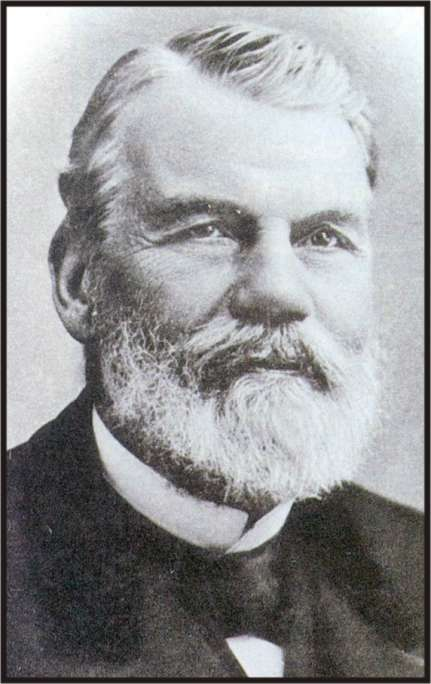
\includegraphics[width=\linewidth]{images/book3/raoult.jpg}
\end{minipage}\hfill
\begin{minipage}[t]{0.76\linewidth}\vspace{0pt}
François-Marie Raoult (1830--1901), professor de química em Grenoble,
mediu, durante a década de 1880, os pontos de congelamento e depois as
pressões de vapor de centenas de soluções, e constatou que, em soluções
diluídas, o abaixamento depende do número de moléculas dissolvidas e não
de sua natureza. Suas medidas se tornaram um meio de pesar moléculas e
sustentaram a jovem teoria dos íons em solução. (Fotografia: domínio
público, Wikimedia Commons.)
\end{minipage}
\end{history}

\section{Misturas reais}

\begin{definition}[Coeficiente de atividade]\label{def:b2:chemical-potential:activity-coefficient}
Em uma mistura real, o \omterm{def:b2:chemical-potential:chemical-potential}{potencial químico} se escreve $\mu_i = \mu_i^\circ +
RT\ln a_i$ com $a_i = \gamma_i x_i$ (referência de Raoult) ou $a_i = \gamma_i
c_i/c^\circ$ (referência de Henry). O fator $\gamma_i$ é o \emph{coeficiente
de atividade}\index{coeficiente de atividade}: ele mede o afastamento da
lei ideal e tende a 1 no limite em que a lei de referência vale.
\end{definition}

Um coeficiente maior que 1 significa que a molécula é menos estabilizada
por suas vizinhas na mistura do que no estado de referência (desvio
positivo, como na figura acima); menor que 1, mais estabilizada. Por
Gibbs--Duhem, os coeficientes dos dois constituintes de uma mistura binária
estão ligados: no modelo de um parâmetro usado na figura, $\ln\gamma_1 = Ax_2^2$
e $\ln\gamma_2 = Ax_1^2$, e
$x_1\,\dd\ln\gamma_1 + x_2\,\dd\ln\gamma_2 = 0$ vale identicamente.

Para os íons, que interagem a longa distância, os afastamentos aparecem já
em concentrações pequenas.

\begin{definition}[Força iônica]\label{def:b2:chemical-potential:ionic-strength}
A \emph{força iônica}\index{forca ionica@força iônica} de uma solução é $I =
\frac12\sum_i z_i^2\,b_i$, em que $b_i$ é a molalidade do íon $i$ (quantidade
por quilograma de solvente) e $z_i$ seu número de carga.
\end{definition}

\begin{proposition}[Lei limite de Debye--Hückel]\label{prop:b2:chemical-potential:debye-huckel}
Em uma solução de eletrólito muito diluída, o \omterm{def:b2:chemical-potential:activity-coefficient}{coeficiente de atividade} médio
dos íons de um sal obedece a $\log\gamma_\pm = -A\,|z_+z_-|\sqrt{I/b^\circ}$, com $A
\approx 0.51$ para a água a \qty{25}{\celsius} e $b^\circ =
\qty{1}{mol/kg}$.
\end{proposition}
\admitted

\begin{remark}[Alcance e origem]\label{rem:b2:chemical-potential:dh-range}
A lei vem de um modelo no qual cada íon é cercado por uma ``atmosfera''
difusa de carga oposta, que abaixa seu \omterm{def:b2:chemical-potential:chemical-potential}{potencial químico}; o modelo está
além deste curso, mas sua constante $A$ decorre da permissividade e da
massa específica da água e da temperatura. Ela é precisa abaixo de cerca de
$I = \qty{0.01}{mol/kg}$. A mesma atmosfera iônica freia os íons em um
campo elétrico e explica por que a condutividade molar de um eletrólito
forte cai segundo $\Lambda = \Lambda^\circ - K\sqrt c$ (lei da raiz
quadrada de Kohlrausch) em vez de ficar em seu valor limite: o limite da
lei de Kohlrausch vista no volume do 1.º ano.
% ledger: epsr:H2O, rho:water.298, const:e, const:eps0, const:kB, const:NA (A computed in figdata/bachelor-2/colligative.py)
\end{remark}

\begin{example}[Um sal centimolar]\label{ex:b2:chemical-potential:dh}
Para o cloreto de sódio a $b = \qty{0.010}{mol/kg}$, $I = \frac12(0.010 + 0.010)
= \qty{0.010}{mol/kg}$ e $\log\gamma_\pm = -0.51 \times 0.10$: $\gamma_\pm
= 0.89$. Já a um centésimo de mol por quilograma, tomar a concentração pela
atividade é um erro de 11\,\%; para um sal 2:2 como o sulfato de magnésio
na mesma molalidade, $I = 0.040$ e $\gamma_\pm = 0.62$.
\end{example}

\section{Propriedades coligativas}

\begin{definition}[Propriedade coligativa]\label{def:b2:chemical-potential:colligative}
Uma \emph{propriedade coligativa}\index{propriedade coligativa} de uma solução
diluída é uma propriedade que depende da quantidade de partículas
dissolvidas por quantidade de solvente e não de sua natureza: o abaixamento
da pressão de vapor e do ponto de congelamento, a elevação do ponto de
ebulição e a \omterm{def:b2:chemical-potential:osmotic-pressure}{pressão osmótica}. As constantes das leis do ponto de
congelamento e do ponto de ebulição abaixo são a \emph{constante
crioscópica}\index{constante crioscopica@constante crioscópica} $K_f$
e a \emph{constante ebulioscópica}\index{constante ebulioscopica@constante ebulioscópica} $K_b$ do
solvente.
\end{definition}

\begin{omfigure}
\begin{tikzpicture}[font=\small, >={Stealth}]
  \draw[->] (0,0) -- (8,0) node[right] {$T$};
  \draw[->] (0,0) -- (0,4.4) node[above] {$\mu$ do solvente};
  % slopes = -S_m: the liquid, more disordered, falls faster than the solid
  \draw[omDef, very thick] (0.4,3.0) -- (7.0,2.01) node[right] {sólido};
  \draw[omThm, very thick] (0.4,3.6) -- (7.6,0.72) node[right] {líquido puro};
  \draw[omThm, very thick, dashed] (0.4,3.25) -- (7.6,0.37) node[right] {solução};
  \fill (2.8,2.64) circle (1.5pt);
  \fill (1.4,2.85) circle (1.5pt);
  \draw[densely dotted] (2.8,2.64) -- (2.8,0) node[below] {$T_f^*$};
  \draw[densely dotted] (1.4,2.85) -- (1.4,0) node[below] {$T_f$};
  \draw[<->] (1.4,-0.75) -- (2.8,-0.75) node[midway, below] {$\Delta T_f$};
  \draw[<->, black!70] (5.0,1.76) -- (5.0,1.41);
  \draw[black!50] (5.0,1.58) -- (4.6,0.75) node[below, font=\scriptsize, black] {$RT\ln x_1$};
\end{tikzpicture}

{\small \omterm{def:b2:chemical-potential:chemical-potential}{Potencial químico} do solvente em função da temperatura (esquema, a
pressão fixa). A fase estável é a de menor $\mu$. Dissolver um soluto abaixa
a reta do líquido de $RT\ln x_1 < 0$; ela passa a encontrar a reta do sólido
a uma temperatura mais baixa: a solução congela abaixo do solvente puro.}
\end{omfigure}

\begin{theorem}[Abaixamento do ponto de congelamento]\label{thm:b2:chemical-potential:cryoscopy}
Uma solução diluída de um soluto que não entra no sólido começa a congelar
em $T_f = T_f^* - \Delta T_f$, com
\[
  \Delta T_f = K_f\,b, \qquad K_f = \frac{R\,T_f^{*2}\,M_1}{\Delta_{\text{fus}}H_1} ,
\]
sendo $b$ a molalidade total das partículas dissolvidas e $M_1$ a massa
molar do solvente (em \unit{kg/mol}). Para concentrações finitas, a relação
exata para uma solução ideal é $\ln x_1 = -\frac{\Delta_{\text{fus}}H_1}{R}
\left(\frac{1}{T_f} - \frac{1}{T_f^*}\right)$.
\end{theorem}

\begin{proof}
No ponto de congelamento, o solvente sólido puro e o solvente na solução
estão em equilíbrio: $\mu_1^{\text{s}}(T) = \mu_1^{*\text{l}}(T) + RT\ln x_1$,
logo $\ln x_1 = -\Delta_{\text{fus}}G_1(T)/(RT)$, com $\Delta_{\text{fus}}G_1 =
\mu_1^{*\text{l}} - \mu_1^{\text{s}}$, nula em $T_f^*$. Por Gibbs--Helmholtz,
$\dd(\Delta_{\text{fus}}G_1/T)/\dd T = -\Delta_{\text{fus}}H_1/T^2$;
integrar de $T_f^*$ a $T_f$ com $\Delta_{\text{fus}}H_1$ constante dá a
relação exata. Para uma solução diluída, $\ln x_1 = \ln(1 - x_2) \approx
-x_2$ e $\frac1{T_f} - \frac1{T_f^*} \approx -\Delta T_f/T_f^{*2}$, logo
$x_2 = \Delta_{\text{fus}}H_1\Delta T_f/(RT_f^{*2})$; por fim, $x_2 \approx
n_2/n_1 = b\,M_1$.
\end{proof}

\begin{proposition}[Elevação do ponto de ebulição]\label{prop:b2:chemical-potential:ebullioscopy}
Uma solução diluída de um soluto não volátil ferve a $T_b^* + \Delta T_b$, com
$\Delta T_b = K_b\,b$, $K_b = RT_b^{*2}M_1/\Delta_{\text{vap}}H_1$.
\end{proposition}

\begin{proof}
O mesmo raciocínio, com o vapor no lugar do sólido: $\mu_1^{*\text{l}} +
RT\ln x_1 = \mu_1^{\text{v}}$; a reta do solvente é abaixada e passa a
encontrar a reta do vapor a uma temperatura mais alta.
\end{proof}

\begin{example}[A água]\label{ex:b2:chemical-potential:water-constants}
Com $\Delta_{\text{fus}}H = \qty{333.4}{J/g} = \qty{6.007}{kJ/mol}$ a
\qty{273.15}{K}: $K_f = 8.314 \times 273.15^2 \times 0.018015/6007 =
\qty{1.86}{K.kg/mol}$. Com $\Delta_{\text{vap}}H = \qty{40.65}{kJ/mol}$ a
\qty{373.12}{K}: $K_b = \qty{0.513}{K.kg/mol}$. Água do mar, \qty{35}{g} de sal
por quilograma, contado como cloreto de sódio (duas partículas por fórmula):
$b = 2 \times 35/58.44/0.965 = \qty{1.24}{mol/kg}$; a lei das soluções
diluídas prevê então \qty{-2.3}{\celsius}, uma superestimativa: nessa
concentração, os íons estão longe do comportamento ideal, e o sal marinho
não é todo cloreto de sódio.
% ledger: dfus:H2O, tfus:H2O, dvap:H2O.nbp, tb:H2O.atm, sea:salinity (computed in figdata/bachelor-2/colligative.py)
\end{example}

\begin{definition}[Membrana semipermeável, pressão osmótica]\label{def:b2:chemical-potential:osmotic-pressure}
Uma \emph{membrana semipermeável}\index{membrana semipermeavel@membrana semipermeável} deixa passar o
solvente e não o soluto. Quando ela separa uma solução do solvente puro,
o solvente flui para a solução; a \emph{pressão
osmótica}\index{pressao osmotica@pressão osmótica} $\Pi$ é o excesso de pressão que é preciso
aplicar à solução para deter esse fluxo.
\end{definition}

\begin{theorem}[Lei osmótica de van 't Hoff]\label{thm:b2:chemical-potential:osmosis}
Para uma solução diluída, $\Pi = c\,RT$, em que $c$ é a concentração total das
partículas de soluto.
\end{theorem}

\begin{proof}
No equilíbrio, o solvente tem o mesmo \omterm{def:b2:chemical-potential:chemical-potential}{potencial químico} dos dois lados:
$\mu_1^*(T, p) = \mu_1^*(T, p + \Pi) + RT\ln x_1$. Como $(\partial\mu_1^*/
\partial p)_T = V_{m,1}$, quase constante para um líquido, $\mu_1^*(T, p + \Pi) -
\mu_1^*(T, p) = \Pi V_{m,1}$, logo $\Pi V_{m,1} = -RT\ln x_1 \approx RT x_2
\approx RT\,n_2/n_1$. Com $n_1V_{m,1} \approx V$ (solução diluída), $\Pi = n_2RT/V$.
\end{proof}

\begin{omfigure}
\begin{tikzpicture}[font=\small, >={Stealth}]
  \begin{scope}
    \clip (-0.85,2.8) -- (-0.85,0.85) arc[start angle=180, end angle=360,
      radius=0.85] -- (0.85,2.8) -- (0.55,2.8) -- (0.55,0.85)
      arc[start angle=0, end angle=-180, radius=0.55] -- (-0.55,2.8) -- cycle;
    \fill[omDef!18] (-1,0) rectangle (0,1.6);
    \fill[omThm!22] (0,0) rectangle (1,2.3);
  \end{scope}
  \pic at (0,0) {utube={0}{white}};
  \draw[very thick, dashed] (0,-0.05) -- (0,0.36);
  \node[left] at (-1.0,1.2) {água pura};
  \node[right] at (1.0,0.9) {solução};
  \draw[densely dotted] (-0.55,1.6) -- (1.55,1.6);
  \draw[densely dotted] (0.85,2.3) -- (1.55,2.3);
  \draw[<->, thick] (1.45,1.6) -- (1.45,2.3) node[midway, right] {$h$, com $\Pi = \rho g h$};
  \draw (0,0.12) -- (0.6,-0.5) node[below right] {membrana semipermeável};
  \draw[->, omDef, thick] (-0.75,0.4) to[bend right=30] (-0.25,0.12);
\end{tikzpicture}

{\small Osmose em um tubo em U. A água atravessa a membrana em direção à
solução até que a pressão hidrostática adicional da coluna mais alta se
iguale à \omterm{def:b2:chemical-potential:osmotic-pressure}{pressão osmótica}; então os \omterm{def:b2:chemical-potential:chemical-potential}{potenciais químicos} da água dos dois
lados são iguais.}
\end{omfigure}

\begin{method}[Massa molar por uma propriedade coligativa]\label{met:b2:chemical-potential:molar-mass}
\begin{enumerate}
  \item Dissolva uma massa conhecida $m_2$ da substância em uma massa conhecida $m_1$
        de solvente (ou em um volume conhecido $V$ de solução).
  \item Meça $\Delta T_f$ (ou $\Delta T_b$, ou $\Pi$).
  \item Deduza a molalidade $b = \Delta T_f/K_f$ (ou $c = \Pi/RT$), depois $n_2 =
        b\,m_1$ (ou $cV$) e $M_2 = m_2/n_2$; divida pelo número de
        partículas por fórmula se a substância se dissocia.
\end{enumerate}
A osmometria convém às moléculas grandes (proteínas, polímeros): alguns gramas
por litro de uma proteína de \qty{60}{kg/mol} dão algumas centenas de pascals,
milímetros de água, mas uma variação do ponto de congelamento de apenas
alguns milésimos de kelvin.
\end{method}

\section{Exercícios}

\begin{exercise}[$\star$]\label{exo:b2:chemical-potential:1}
Use a construção da tangente na figura do volume molar (mistura modelo)
em $x_2 = 0.4$ para ler $\bar V_1$ e $\bar V_2$, e verifique que
$x_1\bar V_1 + x_2\bar V_2$ é o volume molar da mistura.
\end{exercise}

\begin{exercise}[$\star$]\label{exo:b2:chemical-potential:2}
A \qty{25}{\celsius}, a pressão de vapor da água é \qty{3.17}{kPa}.
Calcule, pela \omterm{thm:b2:chemical-potential:raoult}{lei de Raoult}, a pressão de vapor acima de uma solução de
\qty{1.00}{mol} de sacarose (não volátil) em \qty{1.00}{kg} de água.
% ledger: pvap:H2O.298
\end{exercise}

\begin{exercise}[$\star$]\label{exo:b2:chemical-potential:3}
Calcule a concentração de dioxigênio dissolvido na água em equilíbrio com
o ar a \qty{1.013}{bar} e \qty{25}{\celsius} ($H(\ce{O2}) =
\qty{1.3e-5}{mol/(m^3.Pa)}$, \qty{20.95}{\percent} de dioxigênio), em
\unit{mol/L} e \unit{mg/L}.
% ledger: henry:O2, air:O2
\end{exercise}

\begin{exercise}[$\star$]\label{exo:b2:chemical-potential:4}
Para \ce{N2(g) + 3H2(g) <=> 2NH3(g)} a \qty{298}{K}, $\Delta_r G^\circ =
\qty{-32.8}{kJ/mol}$. Calcule $\Delta_r G$ em uma mistura em que
$p(\ce{N2}) = \qty{1.0}{bar}$, $p(\ce{H2}) = \qty{0.010}{bar}$ e
$p(\ce{NH3}) = \qty{1.0}{bar}$, e diga em que sentido a reação ocorre.
\end{exercise}

\begin{exercise}[$\star\star$]\label{exo:b2:chemical-potential:5}
Em uma mistura binária, o \omterm{def:b2:chemical-potential:partial-molar}{volume parcial molar} do constituinte 1 varia de
$\dd\bar V_1 = \qty{-0.30}{mL/mol}$ quando $x_2$ passa de 0.30 a 0.31. Usando
Gibbs--Duhem, encontre $\dd\bar V_2$.
\end{exercise}

\begin{exercise}[$\star\star$]\label{exo:b2:chemical-potential:6}
O soro fisiológico contém \qty{9.0}{g} de cloreto de sódio por litro.
Calcule sua \omterm{def:b2:chemical-potential:osmotic-pressure}{pressão osmótica} a \qty{37}{\celsius}, considerando o sal
totalmente dissociado, e explique por que as hemácias mantêm sua forma
nele, mas incham e se rompem na água pura.
\end{exercise}

\begin{exercise}[$\star\star$]\label{exo:b2:chemical-potential:7}
Uma solução de \qty{2.00}{g} de uma proteína em \qty{100.0}{mL} de água tem
\omterm{def:b2:chemical-potential:osmotic-pressure}{pressão osmótica} de \qty{0.825}{kPa} a \qty{25}{\celsius}. Calcule a massa
molar da proteína e o abaixamento do ponto de congelamento dessa solução.
\end{exercise}

\begin{exercise}[$\star\star$]\label{exo:b2:chemical-potential:8}
Calcule a \omterm{def:b2:chemical-potential:ionic-strength}{força iônica} e os \omterm{def:b2:chemical-potential:activity-coefficient}{coeficientes de atividade} médios (lei limite)
de: (a) cloreto de sódio a \qty{1.0e-3}{mol/kg}; (b) cloreto de cálcio a
\qty{1.0e-3}{mol/kg}; (c) sulfato de magnésio a \qty{1.0e-3}{mol/kg}.
\end{exercise}

\begin{exercise}[$\star\star$]\label{exo:b2:chemical-potential:9}
Uma solução de \qty{1.50}{g} de um composto desconhecido, não volátil e que
não se dissocia, em \qty{50.0}{g} de água congela a \qty{-0.310}{\celsius}.
Calcule sua massa molar.
\end{exercise}

\begin{exercise}[$\star\star\star$]\label{exo:b2:chemical-potential:10}
Mostre que, no modelo de um parâmetro $\ln\gamma_1 = Ax_2^2$, $\ln\gamma_2 =
Ax_1^2$, a relação de Gibbs--Duhem é satisfeita e que a \omterm{prop:b2:chemical-potential:henry}{constante de Henry} do
constituinte 1 é $k_{H,1} = p_1^*\mathrm e^A$. Para $A = 1.1$, por que fator
a inclinação de Henry supera a de Raoult?
\end{exercise}

\begin{exercise}[$\star\star\star$]\label{exo:b2:chemical-potential:11}
Explique por que uma lei coligativa exige (a) um soluto não volátil para a
elevação do ponto de ebulição e (b) um soluto que não entre no sólido para o
abaixamento do ponto de congelamento. O que acontece com o ponto de
congelamento de um solvente cujo soluto forma com ele uma solução sólida
ideal na mesma proporção que no líquido?
\end{exercise}

\begin{exercise}[$\star\star\star$]\label{exo:b2:chemical-potential:12}
Um termômetro lê até \qty{0.01}{K}. Calcule a menor molalidade de um soluto
que não se dissocia detectável na água por crioscopia e por ebulioscopia, e
a \omterm{def:b2:chemical-potential:osmotic-pressure}{pressão osmótica} correspondente a \qty{25}{\celsius}. Qual método é o
mais sensível, e por que se usam osmômetros para os polímeros?
\end{exercise}

\section{Problema: O radiador no inverno}

\begin{problem}[{Problema de fim de semana --- uma \omterm{def:b2:chemical-potential:ideal-mixture}{mistura ideal} de água e
etano-1,2-diol, a lei crioscópica e sua constante, o congelamento de um
fluido de arrefecimento e quanto diol mantém um motor líquido a \qty{-20}{\celsius}}]
\label{pb:b2:chemical-potential:1}
O fluido de arrefecimento de um motor é uma mistura de água e etano-1,2-diol
(\ce{HOCH2CH2OH}, $M = \qty{62.07}{g/mol}$, ponto de ebulição \qty{197}{\celsius},
aqui não volátil). Água: $M = \qty{18.015}{g/mol}$, ponto de congelamento
\qty{273.15}{K}, entalpia de fusão \qty{333.4}{J/g}, ponto de ebulição
\qty{373.12}{K} sob \qty{1.013}{bar}, entalpia de vaporização
\qty{40.65}{kJ/mol}, pressão de vapor \qty{3.17}{kPa} a \qty{25}{\celsius}.
A mistura é considerada ideal.
% ledger: tb:glycol, dfus:H2O, tfus:H2O, tb:H2O.atm, dvap:H2O.nbp, pvap:H2O.298

\medskip
\noindent\textbf{Parte I --- A mistura.}
\begin{enumerate}
  \item Escreva o \omterm{def:b2:chemical-potential:chemical-potential}{potencial químico} da água em uma \omterm{def:b2:chemical-potential:ideal-mixture}{mistura ideal}.
  \item Um fluido de arrefecimento contém \qty{30}{\percent} de diol em massa. Calcule as
        quantidades de diol e de água em \qty{100}{g} e a fração molar da
        água.
  \item Calcule a pressão de vapor da água acima desse fluido a
        \qty{25}{\celsius}.
  \item Calcule a molalidade do diol.
  \item Por que se despreza a pressão de vapor do próprio diol?
\end{enumerate}

\medskip
\noindent\textbf{Parte II --- A lei crioscópica.}
\begin{enumerate}[resume]
  \item Escreva a igualdade dos \omterm{def:b2:chemical-potential:chemical-potential}{potenciais químicos} no ponto de congelamento
        do fluido, sendo o sólido gelo puro.
  \item Usando a relação de Gibbs--Helmholtz, deduza $\ln x_1 =
        -\frac{\Delta_{\text{fus}}H}{R}\left(\frac1{T_f} - \frac1{T_f^*}\right)$.
  \item Linearize-a para uma solução diluída e obtenha $\Delta T_f = K_f b$.
  \item Calcule a entalpia molar de fusão da água e $K_f$.
  \item Que hipótese sobre a entalpia de fusão foi feita na integração?
\end{enumerate}

\medskip
\noindent\textbf{Parte III --- O congelamento.}
\begin{enumerate}[resume]
  \item Calcule o ponto de congelamento do fluido a \qty{30}{\percent} com a
        lei das soluções diluídas.
  \item Calcule-o com a relação ideal exata.
  \item Em qual resultado você confia mais, e por que ambos são apenas
        estimativas para um fluido real?
  \item No ponto de congelamento, o que cristaliza?
  \item Resfriado ainda mais, o líquido restante se enriquece em diol. Explique
        por que o gelo continua a se formar a temperaturas cada vez mais baixas.
\end{enumerate}

\medskip
\noindent\textbf{Parte IV --- A ebulição e a meta de inverno.}
\begin{enumerate}[resume]
  \item Calcule o $K_b$ da água.
  \item Calcule a elevação do ponto de ebulição do fluido a \qty{30}{\percent}
        a \qty{1.013}{bar}.
  \item O radiador é pressurizado a \qty{2.0}{bar}. Usando a relação de
        Clausius--Clapeyron da física com a entalpia de vaporização acima,
        estime o ponto de ebulição da água pura a \qty{2.0}{bar}.
  \item O que importa mais no verão, a tampa ou o diol?
  \item Para um fluido líquido até \qty{-20}{\celsius}, calcule a fração
        molar de água exigida pela relação ideal exata.
  \item Converta-a em fração mássica de diol.
  \item Calcule a fração mássica que a lei das soluções diluídas teria dado e
        explique a diferença.
  \item Dê a fração mássica de diol que mantém o fluido líquido até
        \qty{-20}{\celsius} no modelo de \omterm{def:b2:chemical-potential:ideal-mixture}{mistura ideal}.
\end{enumerate}
\end{problem}
